\section{Phenotypic convergence}

For observing the assets dynamic, we are using an expanding window approach, allowing to distinguish the evolution of the clusters.
In fact, for $t=t_0,\ldots,T$, the $p$-dimensional dataset  is projected on the $k$-dimensional space defined by the main factors extracted trough the Factor Analysis applied on the dataset $X_T$. By using this projection instead of a time-varying factor model, we are avoiding situations like changes in factors loadings, causing inconsistencies over time.
In order to derive the dynamics of the assets’ universe, we used an expanding window approach. The 23-dimension dataset is estimated first for the time interval $[1,t_0]$=[10/10/2014, 02/19/2016]. Then, the time window is extended on a daily basis, up to $T$=10/16/2018 and for each step in time, the 23-dimension dataset is projected on the 2-dimension space defined by the tail factor and the moment factor, estimated for the entire time period.\\
\indent \hyperref[fig:figure_10]{Figure 10} presents a snapshot of the evolution of the assets universe using the expanding window approach.

\begin{figure}[H]
	\begin{minipage}[b]{0.55\textwidth}
	\centering
	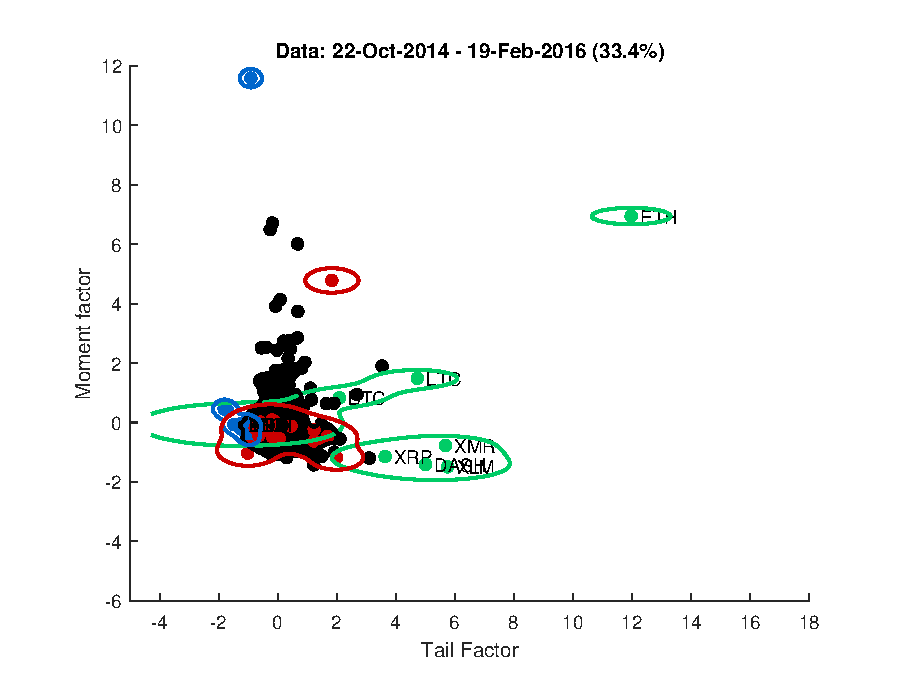
\includegraphics[width=1\textwidth]{Fig/figure_10a}
	
\end{minipage}
\begin{minipage}[b]{0.55\textwidth}
	\centering
	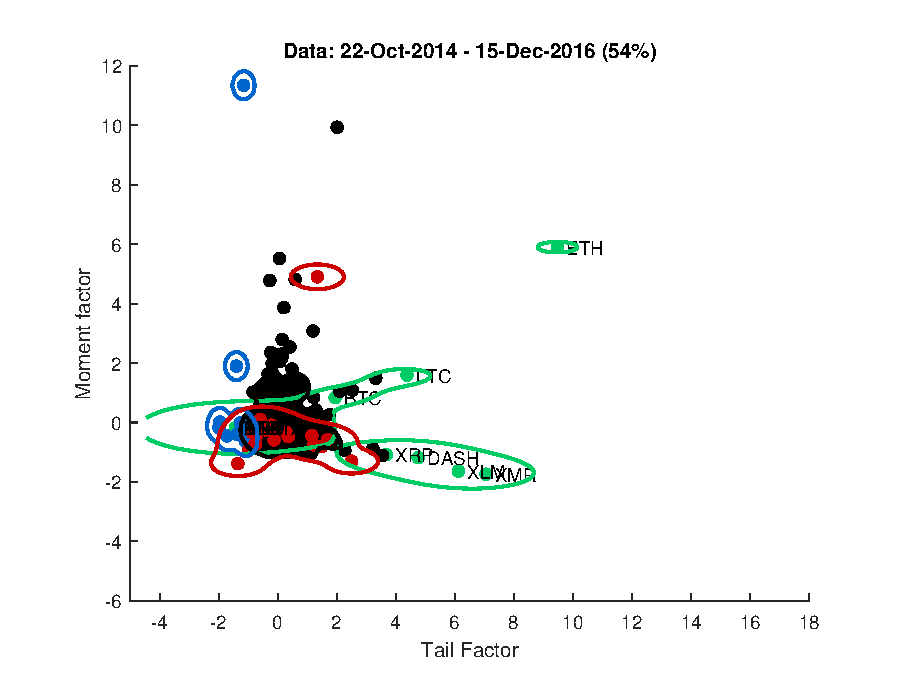
\includegraphics[width=1\textwidth]{Fig/figure_10b}
	
\end{minipage}

	\begin{minipage}[b]{0.55\textwidth}
	\centering
	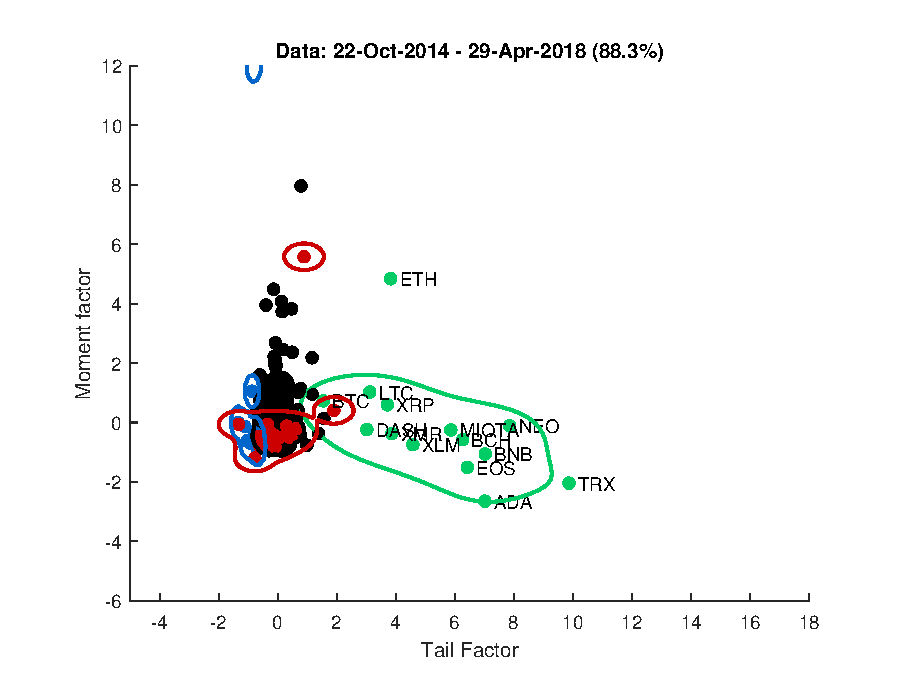
\includegraphics[width=1\textwidth]{Fig/figure_10c}
	
\end{minipage}
\begin{minipage}[b]{0.55\textwidth}
	\centering
	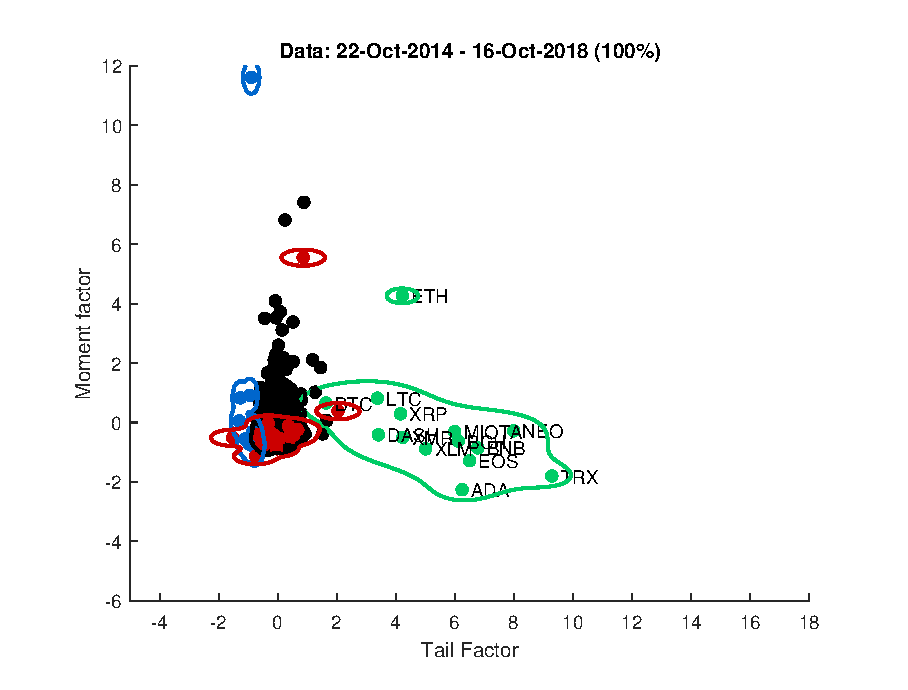
\includegraphics[width=1\textwidth]{Fig/figure_10d}
	
\end{minipage}
	\caption{The evolution of the assets universe using the expanding window approach. The colour code is the following: green - cryptocurrencies, black – stocks, red – commodities, blue – exchange rates\href{https://github.com/QuantLet/Genus_proximum_cryptos/tree/master/DFA_Cryptos}{. DFA\_cryptos.}}
	\label{fig:figure_10}
\end{figure}
The daily evolution of the assets universe, for the period 02/19/2016-10/16/2018 is depicted in this \href{run:Fig/Crypto_movie.mp4}{movie}.\\
\indent{} Looking at the evolution of the assets universe, it appears that the behaviour of cryptocurrencies is a dialectical one and can be described by the concepts of phenotypic convergence and divergent evolution.
These concepts refer to the fact that individual cryptocurrencies tend to develop over time similar certain characteristics (phenotypic convergence) that make them fully distinguishable from the classical assets (divergent evolution).\\
In order to test this behaviour, we are using the Likelihood Ratio associated to model  \ref{form:logit}, estimated using the expanding window approach previously described.
Thus, the Likelihood Ratio of the model \ref{form:logit} can be defined as:
\begin{align} \label{form:conv_lr}
LR(\widehat{\boldsymbol{\beta}})=-2 (\log L(\widehat{\boldsymbol{\beta}})- \log L(\widehat{\boldsymbol{\beta_s}})),
\end{align}
where $L(\widehat{\boldsymbol{\beta_s}})$ is the likelihood of a saturated model that fits perfectly the sample, while  $L(\widehat{\boldsymbol{\beta}})$ is the likelihood of the estimated model.
In the languange of binary logistic regression, the Likelihood Ratio from equation \ref{form:conv_lr} is called deviance \citep{hosmer.2010} and is a measure of model goodness-of-fit, large values indicating models with poor classification power. The deviance is always positive, being zero only for the perfect fit.\\
In order to derive the statistical significance of the classification, we compare the Likelihood Ratios of the estimated model and of the intercept-only model.\\
Thus, we compute the difference of the likelihood ratios: 
\begin{align} \label{form:dif_dev}
D=[LR(\widehat{\boldsymbol{\beta}})-LR(0)]\sim \chi^{2}(1),
\end{align}
$LR(0)$ being the likelihood ratio of the intercept-only model. 
In fact we are estimating $m$ models, where $m=T-t_0-1=971$ and for each model we report the Likelihood Ratio (\hyperref[fig:figure_11]{Figure 11}) and the p-value associated to equation \ref{form:dif_dev} (see the \hyperref[fig:figure_12]{Figure 12}).
\begin{figure}[H]
	\centering
	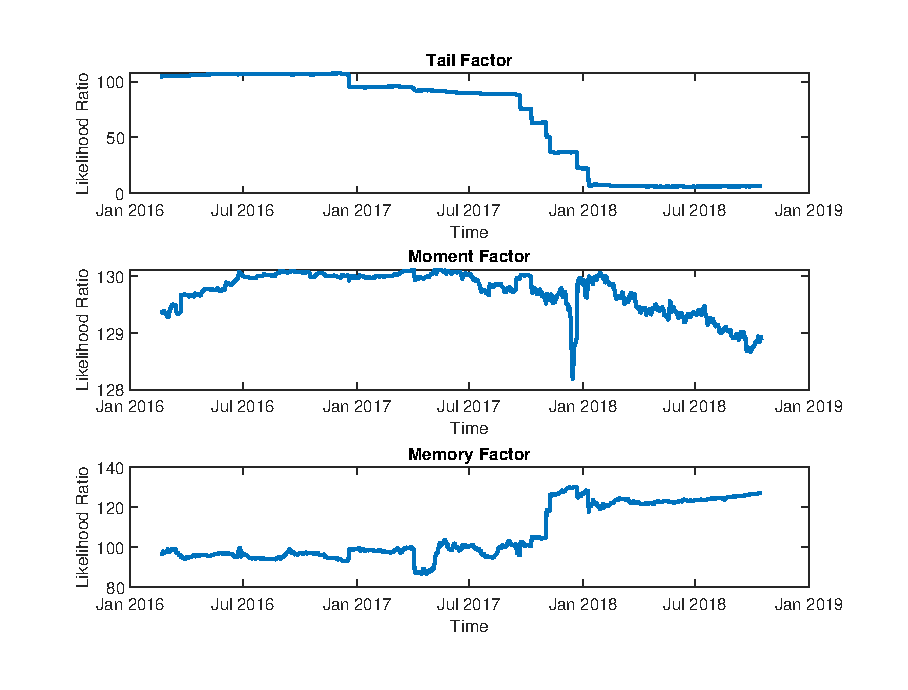
\includegraphics[width=0.85\textwidth]{Fig/figure_11}
	\caption{Likelihood Ratios for the model \ref{form:logit}, estimated for the period 02/19/2016-10/16/2018. \href{https://github.com/QuantLet/Genus_proximum_cryptos/tree/master/CONV_cryptos}{CONV\_cryptos}.}
	\label{fig:figure_11}
\end{figure}
 As shown in \hyperref[fig:figure_11]{Figure 11}, the classification power of the moment and memory factor is negligible, as the Likelihood Ratio is significantly higher than 0.
 However, the model based on the tail factor has an improving goodness-of-it over time, the Likelihood Ratio converging to lower values regime. This result is augmented by the evolution of P-values, shown in \hyperref[fig:figure_12]{Figure 12}: the tail factor is the only one able to discriminate between the cryptocurrencies and classical assets.
 \begin{figure}[H]
 	\centering
 	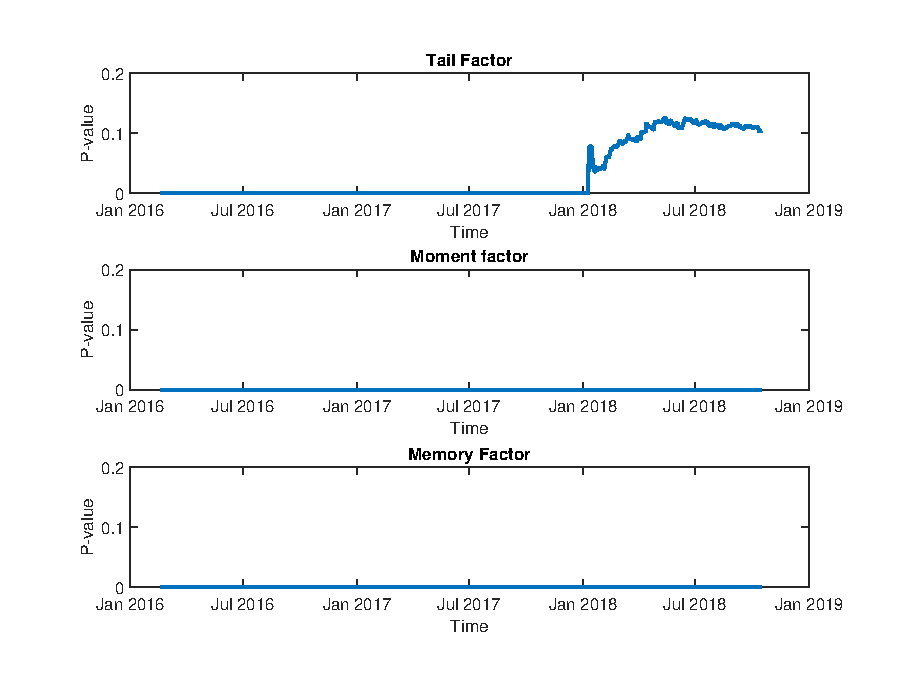
\includegraphics[width=0.85\textwidth]{Fig/figure_12}
 	\caption{P-values for the equation \ref{form:dif_dev}, estimated for the period 02/19/2016-10/16/2018. \href{https://github.com/QuantLet/Genus_proximum_cryptos/tree/master/CONV_cryptos}{CONV\_cryptos}.}
 	\label{fig:figure_12}
 \end{figure}


 By looking the the evolution of the P-values, we can observe that the shift in significance for the tail factor based model is recorded on January 2018, when the cryptocurrencies market collapsed, after the historical maximum of Bitcoin from December 2017.\\ 
 \indent{}The most important implication of this finding is the validity of phenotypic convergence among cryptocurrencies: in their evolution, the individual cryptocurrencies have developed similar characteristics (heavier tails, higher volatility, higher propensity to extreme negative returns), that differentiate them from the classical assets and position them as a new, different species in the ecosystem of financial instruments.